\documentclass[a4paper,notitlepage]{article}
\usepackage{ssn-format}
%\drafttrue
\title{Items to be discussed on science requirements on PFS software}
\author{Atsushi Shimono + Naoyuki Tamura}
\date{2013/11/29}

\usepackage{sciops-scireq}

\begin{document}

\SSNID{00003}
\SSNREV{001}
\SSNCATEGORY{ALL}
\SSNChangeRecord{Rev.001 / First Release / 2013--11--29}
\SSNReference{(none)}
\SSNAttachment{(none)}
\SSNWritten{Atsushi Shimono + Naoyuki Tamura}

\ssnhead

\section{Abstract}

This document is to start discussion to collect requirements from the
science team to the PFS software packages. Especially from the survey
operation points of view, what each software component needs to do and
what kind of user interfaces are necessary are expected to be
clarified. In Section 2, current ideas and understandings of possible
styles of PFS surveys at the instrument builders' sides are presented,
and in Section 3 questions and future discussion items are listed so
that replies from the science team to them can be considered as pieces
of the requirements to the software components.

From SDSS, Michael Strauss gave us a presentation titled "SDSS survey
design \& operation: Inputs for PFS".

\section{Reference documents/materials}

\begin{itemize}
 
 \item A presentation by Michael Strauss (Princeton) in the 5th
       collaboration meeting at Sao Paulo, titled ``SDSS survey
       design \& operation: Inputs for PFS'':
       \url{http://sumire.pbworks.com/w/file/fetch/70573145/Strauss_sdss_spectroscopy.pdf}
 \item An overview presentation of the current status of PFS data
       reduction pipeline by Steve Bickerton (Kavli IPMU): 
       \url{http://sumire.pbworks.com/w/file/71220051/pfs-dec2013-dataprod-sum.pptx}
 \item SDSS Data Release website: \url{http://www.sdss.org/dr7/}
 \item A presentation file from LAM about an example of archive system
       for an other survey: 
       \url{http://sumire.pbworks.com/w/file/71220426/vuds_olf_nov13.pptx}
\end{itemize}

\section{PFS Survey Basics}

Some basic features of PFS surveys can be listed as follows:
\begin{itemize}
 \item PFS survey will consist of four sub-surveys having different
       features as exemplified in
       Table.~\ref{tab:sciops-scireq-subsvy}).
 \item Sub-surveys may share fields and/or exposures.
 \item More targets may exist than fiber \# per field, so each field
       may be exposed multiple times, depending on sub-surveys and
       their goals.
 \item Since a large number of fibers are available and the number of
       targets is probably even larger, processes of survey planning,
       execution, and data reduction should be automated as much as
       possible.
\end{itemize}

\begin{table}[htb]
\caption{Requirements per sub-survey (sample; not completed)}
\label{tab:sciops-scireq-subsvy}
\begin{center}
\begin{tabular}{c|c|c|c|c}
conditions & cosmology & GA-LR & GA-MR & galaxy-AGN \\ \hline
\hline
Individual exposure time & 15min & 15min & 15min & 15min \\
\hline
Total integration time per object & 15min & 120min & 180min & 180min \\
\hline
Science target density (\#/arcmin) & ? & ? & ? & ? \\
\hline
Number of sky fibers per field & ? & ? & ? & ? \\
\hline
Distribution of sky fibers over field & ? & ? & ? & ? \\
\hline
Number of calibration stars per field & ? & ? & ? & ? \\
\hline
Distribution of calibration stars over field & ? & ? & ? & ? \\
\hline
 : & : & : & : & : \\
\end{tabular}
\end{center}
\end{table}

\subsection{Processing a Survey}

\subsubsection{Preparation}

Having master catalog(s) of target objects as inputs, fields of which
centers correspond to telescope pointings are output and fibers are then
allocated to targets in each field
(e.g. Figure.~\ref{fig:sciops-scireq-slide-svyexp}). Multiple fiber
allocations may be considered on a single field so that more targets can
be observed. {\it Some rules need to be applied in defining the fields
(i.e. field center \& position angle are chosen) and allocating fibers
to targets, in order to maximize survey observation efficiency.}  In the
fiber allocation, some key instrument features such as collisions of
neighboring fiber positioners and field distortion on the PFI focal
plane will also be taken into account.

\begin{figure}[htb]
  \begin{center}
    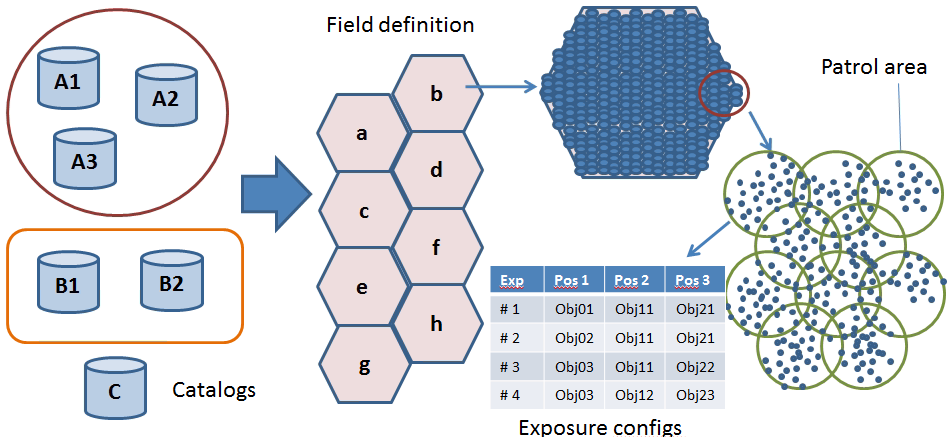
\includegraphics[width=.75\linewidth]{sciops-scireq-slide-svyexp.png}
  \end{center}
  \caption{Schematic view of procedure from list of catalogs to exposure 
    configurations}
  \label{fig:sciops-scireq-slide-svyexp}
\end{figure}

In Figure.~\ref{fig:sciops-scireq-slide-svyexp}, 
each survey (A, B, C) will supply lists of targets (catalogs), 
and some survey might use several lists (e.g. A1, A2, and A3 at left-most 
schematic). 
Using these lists of targets, exposure fields (a, b, c, ...) will be defined 
and targets will be assigned to each field (or more than one field if we 
dither or make overlaps). 
For each field, we will have 2396 circular fiber positioner patrol area 
with some overlapped area (right two schematics). 
We assume to have multiple targets (objects) within each patrol area, 
and software will assign targets into fiber positioners and exposures. 
Some targets requires multiple exposures to complete required exposure time, 
and multiple exposures will be assigned for these targets
(middle bottom table). 

\subsubsection{Observation at the summit}

In Figure.~\ref{fig:sciops-scireq-slide-oneexp}, the basic instrument
operation and data flow in PFS observation is described as a
flowchart. Once the previous exposure is completed, the telescope starts
slewing to the next target field. Using the Acquisition \& Guide (A\&G)
cameras, field acquisition is performed and auto guiding is then
initiated. In parallel to these, fiber configuration is executed, and a
new exposure is started. While CCD detectors are read out only once at
the end of an exposure, IR detector is continuously read out during an
exposure (so-called up-lamp) and outputs a single FITS image at the end
making use of all the data in the intermediate readouts. The FITS data
from the CCD and IR detectors are transferred to Hilo and on-site quick
data reduction process is applied, during the next exposure (see the
Figure.~\ref{fig:sciops-scireq-slide-oneexp}
). Results from this on-site quick data reduction will be transferred to
survey planning \& tracking software (SPT) for records so that the operators
at the summit can check and consider them for subsequent exposures, 
also SPT will check reported data quality assurance data and update survey 
plan for second next exposure from the exposure 
(see also Section.~\ref{sec:qa}). 
Some
more details about the quick and full data reduction pipelines are given
in \S~\ref{datareduction}.

\begin{figure}[htb]
  \begin{center}
    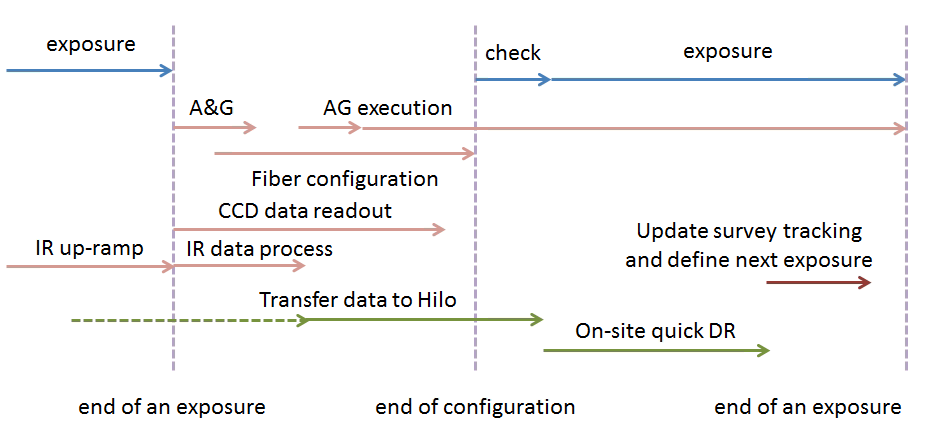
\includegraphics[width=.75\linewidth]{sciops-scireq-slide-oneexp.png}
  \end{center}
  \caption{Activities during observation along timeline}
  \label{fig:sciops-scireq-slide-oneexp}
\end{figure}

%\paragraph{Updating exposure configuration to fit with condition}
%
%Actual observation PA will be defined at the Summit just before each
%exposure, since rotation angle of PFI from the center need to be
%restricted within $\pm$ 60 degree ([TBC]) to make fiber FRD small as
%possible.  We have rotation symmetry by 60 degree on focal plane
%including fiber positioner and A\&G camera, we can rotate PFI by 60
%degree to get the same exposure configuration (excluding individual
%difference among each fiber).  To adjust PA of PFI by rotating integral
%multiplication of 60 degree, we need to update fiber configuration and
%object positions of A\&G and AG with using final settings of PA, to meet
%with small shift per each fiber positioner.  Also ETS need to consider
%of these possible error areas for collision detection among positioners
%during fiber configuration trial.

\subsubsection{Data reduction}
\label{datareduction}

PFS will have two modes of data reduction pipeline (DRP): on-site
quick-look mode, and off-site full mode. The former, which will be
applied to data ``on the fly'' i.e. as they come out in the middle of a
night, will likely be a simplified version of the off-site full DRP. The
full mode will have two functions. One is to reduce a set of data after
each night or each run of a few to several nights to integrate them into
those from the already executed part of the survey. The other is to
periodically do a systematic batch analysis of all the data that have
been already taken.
% But pipeline will be the same for two modes (TBC).

PFS data reduction will be processed roughly as follows (see also
Figure.~\ref{fig:sciops-scireq-drp-slide}): 

\begin{itemize}
  \item 2D extraction of fibers to 1D spectra
  \item Calibration and sky (continuum) subtraction (note: for bright sky 
    emission lines, currently not sure for detail, e.g. 2D PSF deconvolution)
  \item Combine multiple exposures into one spectrum and measure scientific 
    values
\end{itemize}

Details will be described elsewhere (also in a slide attached to this note) 
by the DRP development team (some
already exist in the PDR technical document and presentations in the PDR
and other collaboration meetings).

%Current assumpsions are 
%\begin{itemize}
% \item Host at Hilo, transfer data in parallel or right after submitted%
%    to Gen2
%       \begin{itemize}
%    \item IR (up-ramp) : just transfer finalized image not raw
%          up-ramp, right after end of exposure and image
%          finalization
%    \item other : transfer data right after end of readout
%      \end{itemize}
% \item Calibrate with pre-built data, but not with simultaneous 2D/1D 
%       calibration data (including PSF/FRD)
% \item Process during next exposure, and return data quality metrics (well?) 
%       before beginning of next configuration
% \begin{itemize}
%  \item How we can reduce pipelines will be a trade off between quality 
%        and time of data processing
% \end{itemize}
%\end{itemize}

\subsubsection{Quality assurance (QA) and survey progress tracking}
\label{sec:qa}

%PFS will have an on-site quick data reduction pipeline (DRP) as a simple
%version of the off-site full DRP.
So far we assume that after each single exposure, the quick DRP is
applied 
over the data set acquired by the exposure and pre-defined calibration data 
and some QA process is performed, but {\it QA process has not
been specifically defined yet.}  One example that will likely be
implemented is the measurement of signal-to-noise ratios (S/N) of
spectra of science and calibration targets, but if others are needed,
they should be requested, although what information can be extracted
with good enough accuracy from a single exposure is somewhat unclear at
this moment. Based on the results from on-site quick DRP, observation
strategy may be updated during a run (or even during a night, if
required), but the information that can be obtained is limited by the
capability of quick DRP. Clearly trade studies will be needed by
comparing required information with computational power (processing
time) \footnote{With making computing resources larger, we might be
possible shorten processing time without reducing procedure in some
level..}.

As survey observation progresses, more data are integrated and the
quality of spectra is improved. The quick and full DRPs will send the
information of the quality of existing spectra on a individual object
basis to survey planning and tracking software (SPT). {\it Some criteria
need to be defined judge whether or not enough data have been taken for
single fields and/or individual objects.} Once a single object and/or
field is considered ``done'', subsequent observation strategy
(e.g. field definition, fiber configuration, required number of
exposures, etc) is expected to be updated by SPT.

\begin{figure}[htb]
  \begin{center}
    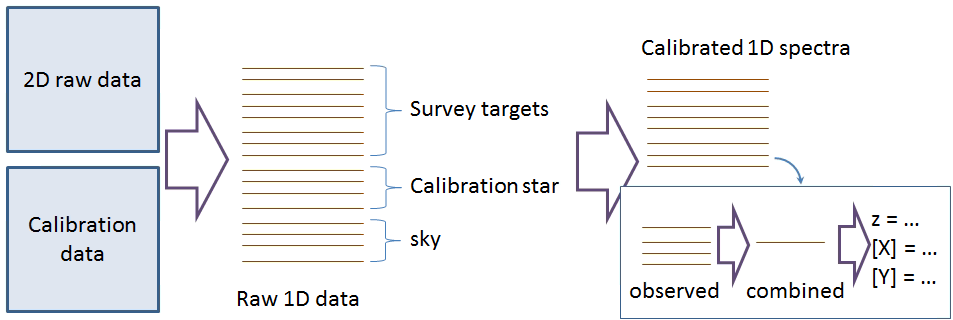
\includegraphics[width=.75\linewidth]{sciops-scireq-drp-slide.png}
  \end{center}
  \caption{Schematic process for PFS data reduction pipeline}
  \label{fig:sciops-scireq-drp-slide}
\end{figure}

\subsection{PFS Software lineup}

To perform all required activities on PFS, PFS software is defined as
four packages and executes a survey as
Figure.~\ref{fig:sciops-scireq-slide-softcoord}:
\begin{description}
 \item[ICS] Instrument Control Software\footnote{So-called ``OBCP'' in
        the Subaru's terminology is a key role of ICS.}
        \begin{itemize}
         \item Everything from observation operation (provided exposure
           configuration) to output raw data.
         \item Including control software directly connected to hardware
         \item Including software for engineering, heartbeat, etc.
        \end{itemize}
 \item[DRP] Data Reduction Pipeline
        \begin{itemize}
         \item Reducing and calibrating raw data for science
         \item On-site quick look DRP, reduced data archive
        \end{itemize}
 \item[ETS] Exposure Targeting Software
        \begin{itemize}
         \item From possible target lists in a single field to fiber
           configuration for a single exposure
         \item Handling coordinate transformation related on sky coordinate
           (within one field)
        \end{itemize}
 \item[SPT] Survey Planning and Tracking software
        \begin{itemize}
         \item From large survey target lists to series of exposures on
           multiple fields
         \item Tracking survey progress including data QA for every
           exposure (by off-site full-DRP)
        \end{itemize}
\end{description}

\begin{figure}[htb]
  \begin{center}
    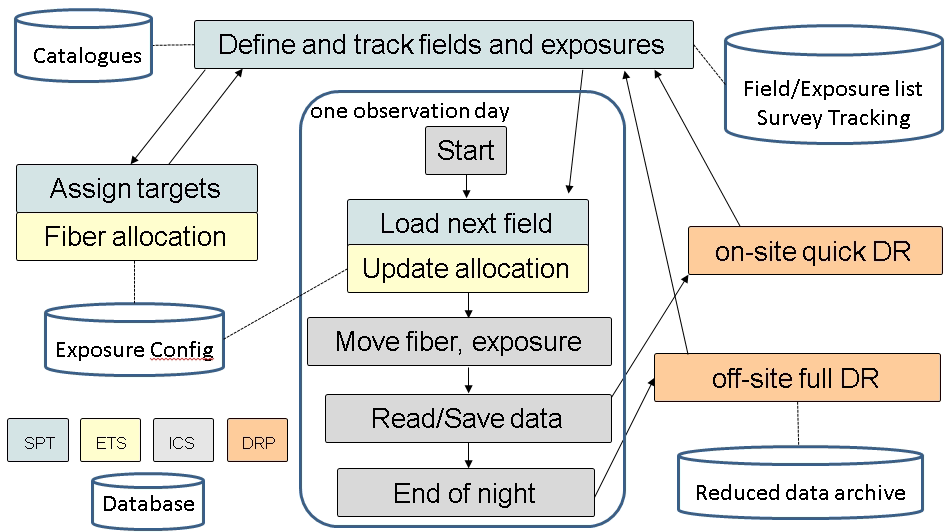
\includegraphics[width=.75\linewidth]{sciops-scireq-slide-softcoord.png}
  \end{center}
  \caption{Sequence of top level activities for entire survey and 
    their associated package}
  \label{fig:sciops-scireq-slide-softcoord}
\end{figure}

From data point of view, each package will handle data or table as
color-coded in Figure.~\ref{fig:sciops-scireq-slide-data}. Supplied
objects by catalogs from science team will be mapped into exposure
field lists. For each exposure field list, multiple exposure
configuration will be created, and results or intermediate outputs will
be attached to each configuration and each field list.  For each
exposure configuration, exposed data and reduced results will be
attached after execution of exposure.

\begin{figure}[htb]
  \begin{center}
    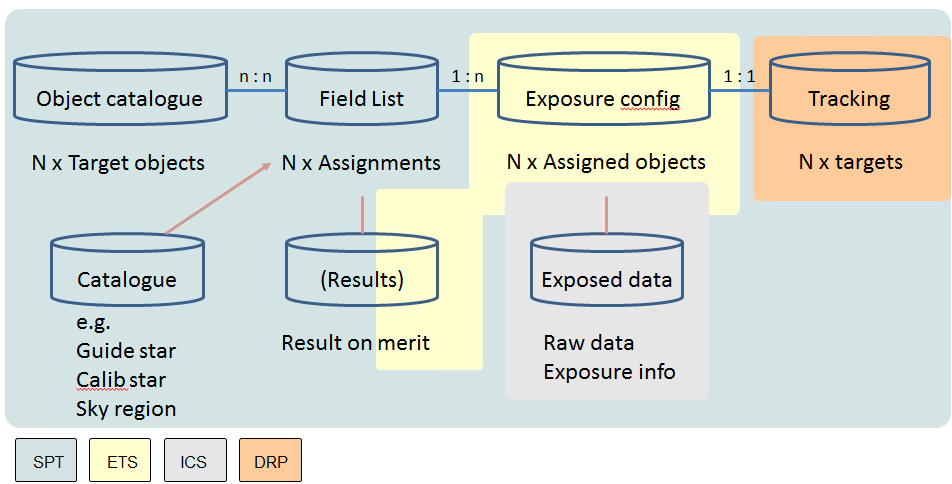
\includegraphics[width=.75\linewidth]{sciops-scireq-slide-data.png}
  \end{center}
  \caption{Relationship between supplied and exposed data from catalog
    to survey tracking data} \label{fig:sciops-scireq-slide-data}
\end{figure}


\clearpage

\section{Questions and Discussion items}

In this section, a list of questions to the science team and future
discussion items are presented, in order to collect requirements needed
to develop the listed software packages.

The priorities \& types of questions/discussion items are color-coded as
follows:
\begin{enumerate}
  \item[\colm{x}] High priority. Replies are requested in a short time
           scale, like 1 month.
  \item[\colm{x}] Less urgent, so please send replies in 6 months.
\end{enumerate}

{\bf Important notes:}
\begin{itemize}
 \item Replies do NOT need to be based on solid plans of your
   surveys. Please tell us current ideas, which should be a good
   starting point of discussion.
       (So, any comment or suggestion is welcome, even not an idea nor reply.) 
 \item Honestly speaking, there may be some important questions and
       discussion items that are missed from this document, so comments
       and additions are welcome.
 \item The format of some questions may not be ideal and therefore may
       not allow you to answer them easily. In such a case, please send
       us your comments and point out why you feel it difficult to
       reply. For example:
       \begin{itemize}
    \item Question is not well understood.
    \item Question is not applicable to my survey.
    \item My survey has different types of requirements such as ... 
    \item ... etc
       \end{itemize}
 \item The questions presented in this document are the first
   set. Your replies to them will then allow us to send you more
   advanced questions. There are a number of subjects which need to be
   iteratively discussed for us to correctly understand requirements
   for relevant implementations.
\end{itemize}

\subsection{Survey basics}

\begin{enumerate}
  \item[\cols{a}] Complete Table~\ref{tab:sciops-scireq-subsvy} by
           checking the numbers that already exist, and giving
           typical numbers to the slots currently occupied by
           ``?''. If ANY corrections and/or additions are necessary,
           please send them to us.
\end{enumerate}

\subsection{Survey preparation}

\subsubsection{Target list}

\begin{enumerate}
 \item[\cols{a}] How would you prepare master catalog(s)?  Please
          include some explanations of your ideas about the key
          issues as listed below:
          \begin{itemize}
           \item Original data or catalog(s) based on which master
             catalog(s) for PFS survey are created
           \item Types of objects to be included. Presumably all
             potential targets not only for science but also for
             calibration, field acquisition, and auto guiding
             (i.e. stars) are included?
           \item Catalog format (number of columns, parameters to be
             listed, etc)
           \item Astrometry (reference star catalog, etc)
           \item Version control of catalog
          \end{itemize}
\end{enumerate}

\subsubsection{Field definition}

\begin{enumerate}
 \item[\cols{a}] How do you want to determine field centers and position
          angles of the fields? Are there any possible optimization
          processes in your mind? Possible examples may be:
          \begin{itemize}
           \item Maximizing the accessibility to high-priority
             science targets
           \item Maximizing the number of stars that can be imaged
             by the A\&G cameras for field acquisition and auto
             guiding.
           \item Uniformizing the number of science targets per
             field.
           \item Pre-defined over entire survey area. 
          \end{itemize}
 \item[\cols{b}] Do you need to visit individual fields multiple times?
          If yes:
          \begin{itemize}
           \item How would you define the number of visits? 
             (e.g. pre-defined number at most, balancing over entire survey 
             area, certain fraction at least) 
           \item Would you keep the field center and position angle
             for all the visits?
          \end{itemize}
 \item[\cols{c}] Do you need to have an overlap between neighboring
          fields? If yes, how would you want to define such an
          overlap?
\end{enumerate}

\subsubsection{Fiber allocation}

For each field (or each exposure), a list of objects need to be selected
from the master catalog(s) and fibers are assigned to them for
integration. In addition to science targets, some fibers will need to be
allocated to calibration stars and blank sky areas. In some cases, you
may also want to mix science targets with other sub-surveys into your
fiber allocation.

\begin{enumerate}
  \item[\cols{a}] Based on what kind of criteria/rules/procedures would
           you like to select science targets to which fibers are
           allocated? Some possible examples are:
           \begin{itemize}
        \item A merit function that is defined by or calculated from 
              a subset of
              parameters in the master catalog.
        \item Priority that is given in advance to individual
              objects or categories of them in the master
              catalog.
           \end{itemize}
  \item[\colm{b}] If you need to visit single field multiple times, how
           would you want to split objects into subsets for the
           multiple visits and determine fiber allocations?
  \item[\colm{c}] How do you want to split fibers into the targets for
           your survey and those for other PFS sub-surveys, if
           required?
%   \begin{itemize}
%     \item When one field or exposure is shared by multiple surveys, we need 
%       to combine two indexes supplied by each survey.
%     \item How to do? Integrate into single merit function, or threshold like 
%       "Survey A index 1 need to be observed up to 80\%", etc.
%    \end{itemize}
  \item[\cols{d}] What type of objects (stars) would you select as
           calibration stars? How many of them will be enough for
           your goals of calibration (See
           Table.~\ref{tab:sciops-scireq-subsvy}), accounting for
           e.g. possibility of cross-check? Any specific
           requirements to their spatial distribution in the field?
           \footnote{PFS software will also query catalog(s) of stars 
           supplied by survey operators, 
           independently from sub-survey catalog(s).} 
  \item[\cols{e}] How would you define ``blank'' sky areas for sky
           fibers? Do you think you can define ``blank'' sky areas
           just based on the information in your master catalog(s)?
  \item[\cols{f}] How do you want to spatially distribute the sky fibers
           in one field?
\end{enumerate}

%\paragraph{Miscellaneous targets}
%
%Definitions of criteria or requirements for miscellaneous targets will 
%vary per each survey, and we need to have a table like 
%Table.~\ref{tab:sciops-scireq-subsvy}. 
%
%\begin{enumerate}
%  \item[a] How many fibers need to be assigned to these targets, including 
%    distribution over a field? 
%  \item[b] Sky fiber positions checked using HSC image or other scheme?
%  \item[c] Calibration star selection criteria: color? intensity? instrument deformation?
%\end{enumerate}

\subsection{Observation execution}

\begin{enumerate}
  \item[\cols{a}] Will you possibly want to visit a certain field
           multiple times in different nights/runs/seasons when it
           is technically feasible?
           Or a certain field need to be visited within a single 
           night/run/season when it is technically feasible? 
           \footnote{Depending on when you
           observe a given area of sky, the positions of target
           objects on the focal plane slightly change due to
           e.g. differential atmospheric refraction, so fiber
           positions need to be adjusted accordingly. The operation
           of the rotator will also be different again depending on
           observing time, due to the $+/-60^{\circ}$ limitation
           (for the sake of minimizing Focal Ratio Degradation (FRD)
           variation, exploiting the hexagonal symmetry of the focal
           plane).}
  \item[\cols{b}] As mentioned in the other parts of this document, we
           expect some QA process is performed and based on the
           information from it observation strategy (e.g. field
           definition, fiber configuration, required number of
           exposures, etc) may be updated. How often would you
           likely want to apply such updates? Should it have to be done
           within the same night \footnote{QA by on-site quick DR will
       be performed during next exposure.}? Or, next nights is OK?
%  \item[\colm{c}] Some survey requires software to stop exposure after certain 
%    signal to noise ratio achieved. 
%    If we expose the same field with the same fiber configuration
%    continuously, we cannot stop by the next exposure after achieval. 
%    How do we do -- prevent such continuous exposure (change every objects 
%    at any time), take survey time efficiency by ignoring such small number of 
%    targets.
\end{enumerate}

%\paragraph{If we dither, rotate or overlap fields}
%
%If field definition is static and almost without gap nor overrap, 
%one target will be mapped into one fiber positioner, and we don't need to 
%care of complex multiple -- multiple assignments. 
%But if not, we might need to care of many things... 
%
%\begin{enumerate}
%  \item[\colm{a}] How many targets we can assume per one fiber positioner patrol 
%    area?
%  \item[b] If we have multiple targets within one fiber positioner patrol 
%    area, set of targets per patrol area will differ field by field 
%    (e.g. target A and B are in area 1 for configuration x, 
%    A in 100 and B in 101 for configuration y). 
%    Survey progress will be complexed and it will take more exposurs to 
%    complete "minimum set", is it ok?
%  \item[c] Do we need to optimize exposure configurations and fiber -- target 
%    assignments over entire survey period or just a exposure by a exposure? 
%\end{enumerate}

\subsection{Data reduction}

%This section covers requirements about data reduction pipeline from raw
%data to reduced 1D spectrum and scientific values extracted from
%spectrum \footnote{Check later section for reduced data and scientific
%values' archive.}. Science requirements including reduction and
%calibration accuracies shall be discussed in separated for two modes.

%\subsubsection{On-site quick DRP}

%\subsubsection{off-site full data reduction pipeline}

%For functional requirements, final output from data reduction pipeline
%will be survey archive data, such as table of astrophysical values,
%reduced data sets (1D spectra and required intermediate outputs). 

%On this point, we need to define what information or output are required
%to be produced:

\begin{enumerate}
 \item[\cols{a}] After a fully reduced and calibrated 1D spectrum is extracted,
      what do you want to measure using the spectral features?
 \item[\cols{b}] Could you briefly explain how you will measure them?
      For example:
      \begin{itemize}
       \item Measure a redshift (or radial velocity) by fitting a
         gaussian to an emission/absorption line (more than one
         lines are fitted simultaneously if available).
      \end{itemize}
 \item[\colm{c}] Do you think there are any special recipes of data reduction 
      and calibration that are needed to the data for your
      (sub-)surveys but are not needed for other surveys?
      Do you think there are any special from 
      current assumed ``normal'' recipes or procedures shown in an 
      attached slide on DRP?  
 \item[\colm{d}] The data reduction and calibration follow many steps, so a
      number of intermediate data will be formed. Are there anything
      specific among them you will likely need/want to access to?
      (e.g. un-wavelength calibrated spectra, spectra without sky subtraction) 
\end{enumerate}

\subsubsection{Data QA and feedback to SPT}

\begin{enumerate}
 \item[\cols{a}] While you are integrating certain objects, to monitor the
      quality of your spectra, what kind of quantities and/or
      diagnostics would you need to see? Earlier in this document,
      S/N (of continuum and/or emission line which may depend on the
      survey objectives) is presented as an example (c.f. integrated
      S/N at SDSS). Is this appropriate, and how do you define S/N 
      (e.g. continuum and/or emission/absorption line at certain wavelength)? 
      Are there any others in
      addition to S/N? Some examples may be:
      \begin{itemize}
       \item Record flux level and noise level separately.
       \item Record fiber positioning errors (residual distances
         from the target positions).
      \end{itemize}
 \item[\colm{b}] Data quality also strongly depends on sky conditions and
      instrument status at individual exposures. What information
      would you specifically want to be recorded?
 \item[\cols{c}] In what criteria should each object be judged ``done''
      (i.e. no more integration is needed)?
 \item[\cols{d}] In what criteria should each field or each fiber configuration
      be judged ``done'' (i.e. no more visit is needed to this
      field/configuration)?
 \item[\cols{e}] The estimation of e.g. S/N by quick DRP is perhaps less
      accurate than full DRP, so more objects may be judged ``done''
      after applying full DRP. Conversely, detailed reduction by
      full DRP may reveal some erroneous features in the data that
      are not detected by quick DRP and some objects may need to be
      ``undone''. So is it correct that you would like to see if
      updates are necessary to observation plans based on not only
      the outputs from on-site quick DRP but also off-site full DRP
      when available?
 \item[\cols{f}] Do you think an automatic release of status/progress
          report per night and/or per run (c.f. Subaru observation
          software system (SOSS) releases a PDF after each night).
\end{enumerate}

\subsection{User interface requirements}

Users approach to software components to access to some data and/or
accomplish some tasks. Once the functional requirements to the software
components are clarified, other requirements such as what data to be
stored and how to visualize them (i.e. user interface requirements) can
be discussed. At this moment, we are trying to understand their
functional requirements by having replies from the science team to the
inquiries presented earlier in this document, so we will only present
the titles of subsections in our mind and will compose the contents with
a list of questions later.

\subsubsection{Preparation}

\subsubsection{Observation execution and data reduction}

\subsubsection{Monitoring of survey progress}

\subsubsection{Interface to ICS}


\subsection{Survey data archive}

\begin{enumerate}
 \item[\cols{a}] What kind of survey archive system do you need/want?
          What would it need to be useful for? Could you tell us
          your ideas, taking care of such key words as follows:
          \begin{itemize}
           \item Data release
           \item Software release
           \item Survey plan \& schedule
           \item Survey progress \& status report
           \item Technical reports
             \begin{itemize}
              \item Instrument performance
              \item Before and after of trouble shooting,
                maintenance work, upgrade, etc
              \item Features in data, tips for
                reduction \& calibration, etc
             \end{itemize}
           \item Public information \& outreach
          \end{itemize}
\end{enumerate}

Below a couple of examples from existing survey archives are presented
as references/starting points of discussion:
\begin{itemize}
 \item SDSS Data Release website: \url{http://www.sdss.org/dr7/}
 \item A presentation file from LAM about an example of archive system
       for an other survey: 
% \item Visualization via kml? 
%   (<kml xmlns="http://www.opengis.net/kml/2.2" hint="target=sky">)
\end{itemize}

\subsection{Data release}

As a background of survey archive, we need to perform continuous data
reduction and periodic re-reduction of full data set.  Single(?) data
reduction after each observation (single day or single run) could be
performed on-premise (or even using on-site DR facility at Hilo supplied
by us, although we need to care about already exposed data set...).  And
this will not be an issue. For continuous data release like a "DR" of
SDSS, Robert Lupton suggested to go cloud. Total "raw" data set will be
around 0.5PB (to 1PB), and even after reduction it will be a level of
1PB including intermediate data.  It could be possible.

\begin{enumerate}
  \item[\cols{a}] Do we need such periodical data release?
  \item[\colm{b}] What do we change on each data release --- pipeline upgrade?
\end{enumerate}


\subsection{Other requirements for calibration}

Any requirements on calibrations?

\begin{enumerate}
  \item[\colm{a}] Statistics of calibration? --- to check stability in short and long 
    term
  \item[\colm{b}] Cross-check by calibrating calibration object by themselves within a 
    frame
\end{enumerate}

\section*{Appendix: System-level requirements associated with data reduction}

Currently, several statistical requirements are already included into
PFS L2 requirements:
\begin{itemize}
  \item REQ-SYS-679, sky subtraction to the accuracy of 0.5\% [TBC] or better 
    of sky
  \item REQ-SYS-896 (890), subtract diffuse background to [TBD] e- accuracy
  \item REQ-SYS-688, flat-field systematics in fibers and detectors to 0.5\% 
    [TBC] or better
  \item REQ-SYS-696, wavelength to 0.01 pixel [TBC] accuracy
  \item REQ-SYS-656, relative flax of individual object spectrum to 5\% [TBC]
    accuracy
\end{itemize}

\end{document}

